\documentclass[hyperref=colorlinks]{beamer}
\mode<presentation>
\usetheme{iclpt}
\setbeamertemplate{navigation symbols}{}
\setbeamertemplate{headline}{
\begin{beamercolorbox}[leftskip=.2cm,rightskip=.2cm,topskip=.2cm,ht=1.1cm,dp=0.1cm,wd=\textwidth]{institute in head/foot}
  
\includegraphics[height=1cm]{icl.pdf}
  \hfill
  
\includegraphics[height=1cm]{../Pics/CMS-Color.pdf}
\end{beamercolorbox}
}
\setbeamertemplate{footline}{
\begin{beamercolorbox}[ht=.55cm,dp=0.4cm,wd=\textwidth,leftskip=.3cm]{author in head/foot}%
  \begin{minipage}[c]{5cm}%
    \usebeamerfont{author in head/foot}
    \insertshortauthor 
    \insertshorttitle
    \end{minipage}\hfill%
  \insertframenumber{} / \pageref{lastframe}
  \hfill
  \begin{minipage}{6cm}
    \hfill
  \end{minipage}
\end{beamercolorbox}%
}

\usepackage{color}
\usepackage{tabularx,colortbl}
\usepackage{graphicx}
\usepackage{pdfpages}
\usepackage{feynmp}
\DeclareGraphicsRule{*}{mps}{*}{}

\title{Lepton Efficiency Uncertainties}
\author[P. Dunne]{P. Dunne}
\date{}
\begin{document}
\begin{fmffile}{feynmandiags}

%TITLE PAGE
\section{Title}
\begin{frame}
  \titlepage

\end{frame}

%OUTLINE
\begin{frame}
  \frametitle{Introductinon}
    \vspace{-0.3cm}
    \vspace{-0.2cm}
    \begin{block}{}
      \footnotesize
      \begin{itemize}
      \item Combinations group asked us to determine whether the lepton ID/veto efficiency uncertainty had an effect on our analysis
      \item Efficiency is not applied in analysis A code
      \item In analysis B it is applied on an event by event per lepton basis the same as in $ZH\rightarrow ll+inv$
      \end{itemize}
    \end{block}
\end{frame}

\begin{frame}
  \frametitle{Method}

        \begin{block}{Tight leptons (Control Regions)}
          \begin{itemize}
          \item For every tight lepton selected weight event by: $\epsilon_{data}/\epsilon_{MC}$
          \end{itemize}
        \end{block}

        \begin{block}{Veto leptons (Signal Region)}
          \begin{itemize}
          \item In selected events there are, by definition, no reconstructed veto leptons
          \item Get generator level leptons in event
          \item Apply a weight of $\frac{1-\epsilon_{data}}{1-\epsilon_{MC}}$ for each gen lepton in the $p_T$ and $\eta$ acceptance
          \end{itemize}
        \end{block}
\end{frame}

\begin{frame}
  \frametitle{Veto Event Weight}
  \begin{columns}
    \column{.5\textwidth}
    \centering
    Electron ($W\rightarrow e\nu$ MC no EWK)
    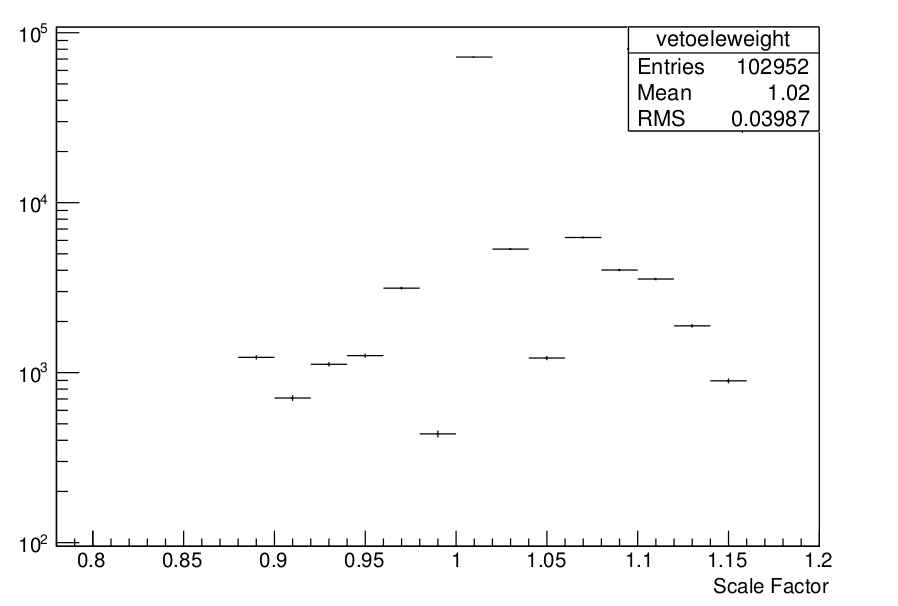
\includegraphics[width=1.1\textwidth]{TalkPics/lepeff141013/croppedvetoeleweight.png}
    \column{.5\textwidth}
    \centering
    Muon ($W\rightarrow\mu\nu$ MC no EWK)
    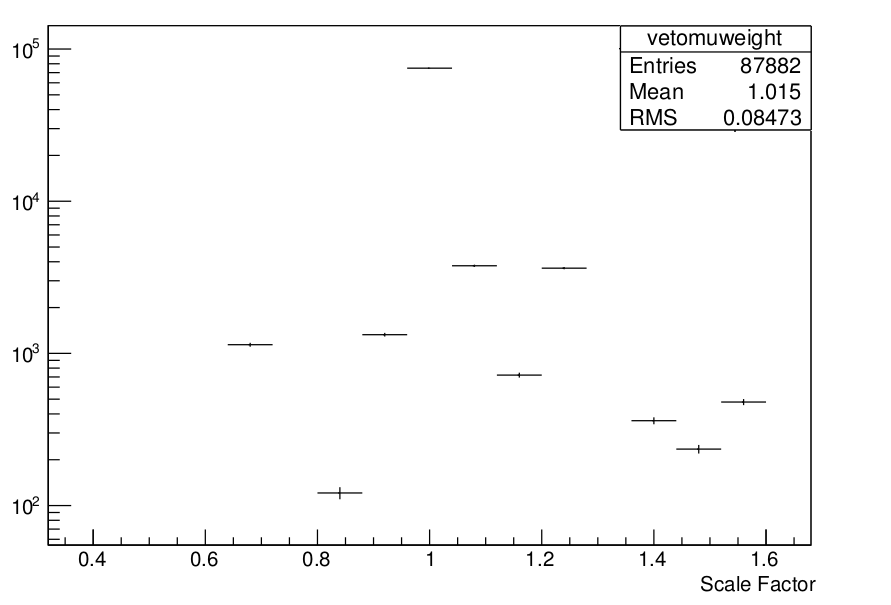
\includegraphics[width=1.1\textwidth]{TalkPics/lepeff141013/croppedvetomuweight.png}
  \end{columns}
  Plots after lepton veto step
\end{frame}

\begin{frame}
  \frametitle{Tight Event Weight}
  \begin{columns}
    \column{.5\textwidth}
    \centering
    Electron ($W\rightarrow e\nu$ MC no EWK)
    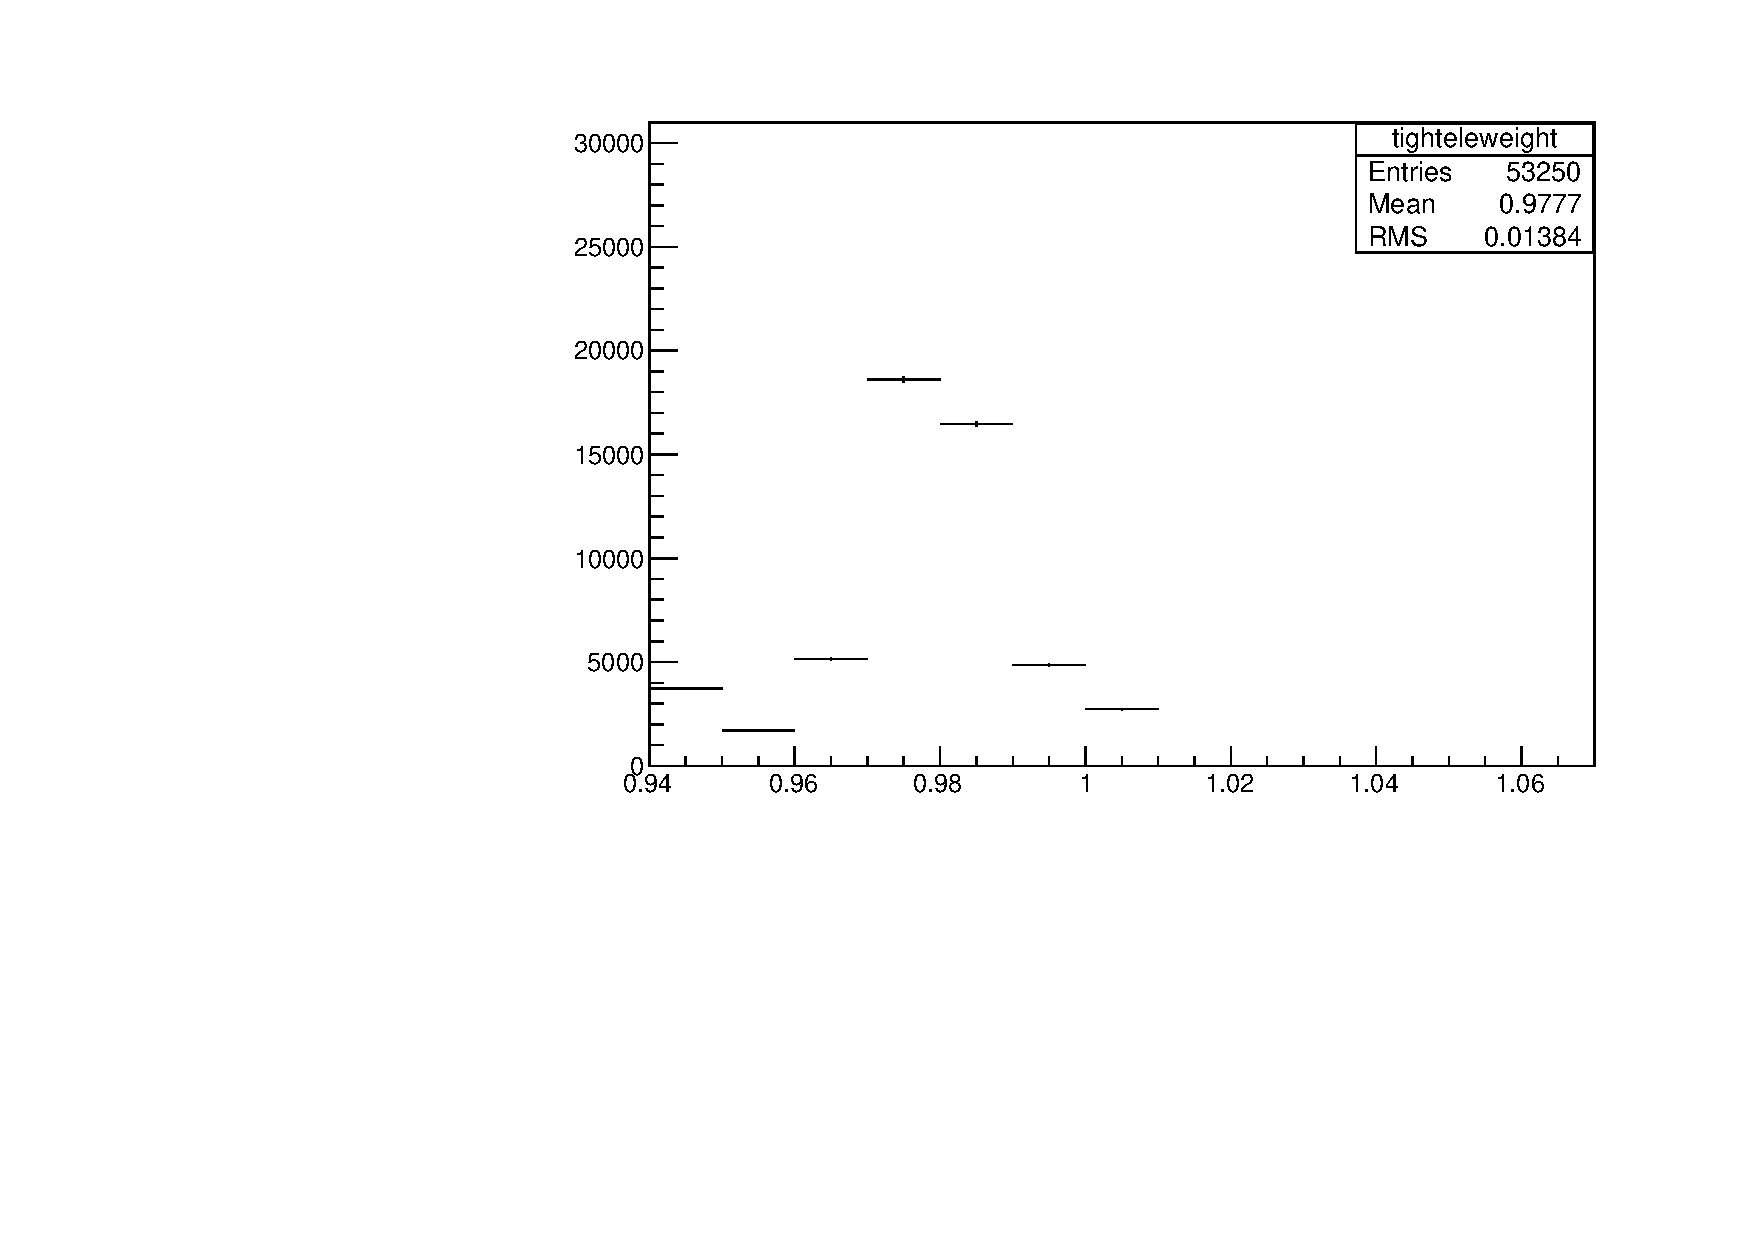
\includegraphics[width=1.1\textwidth]{TalkPics/lepeff141013/tight_eleweight_enu_enu.pdf}
    \column{.5\textwidth}
    \centering
    Muon ($W\rightarrow\mu\nu$ MC no EWK)
    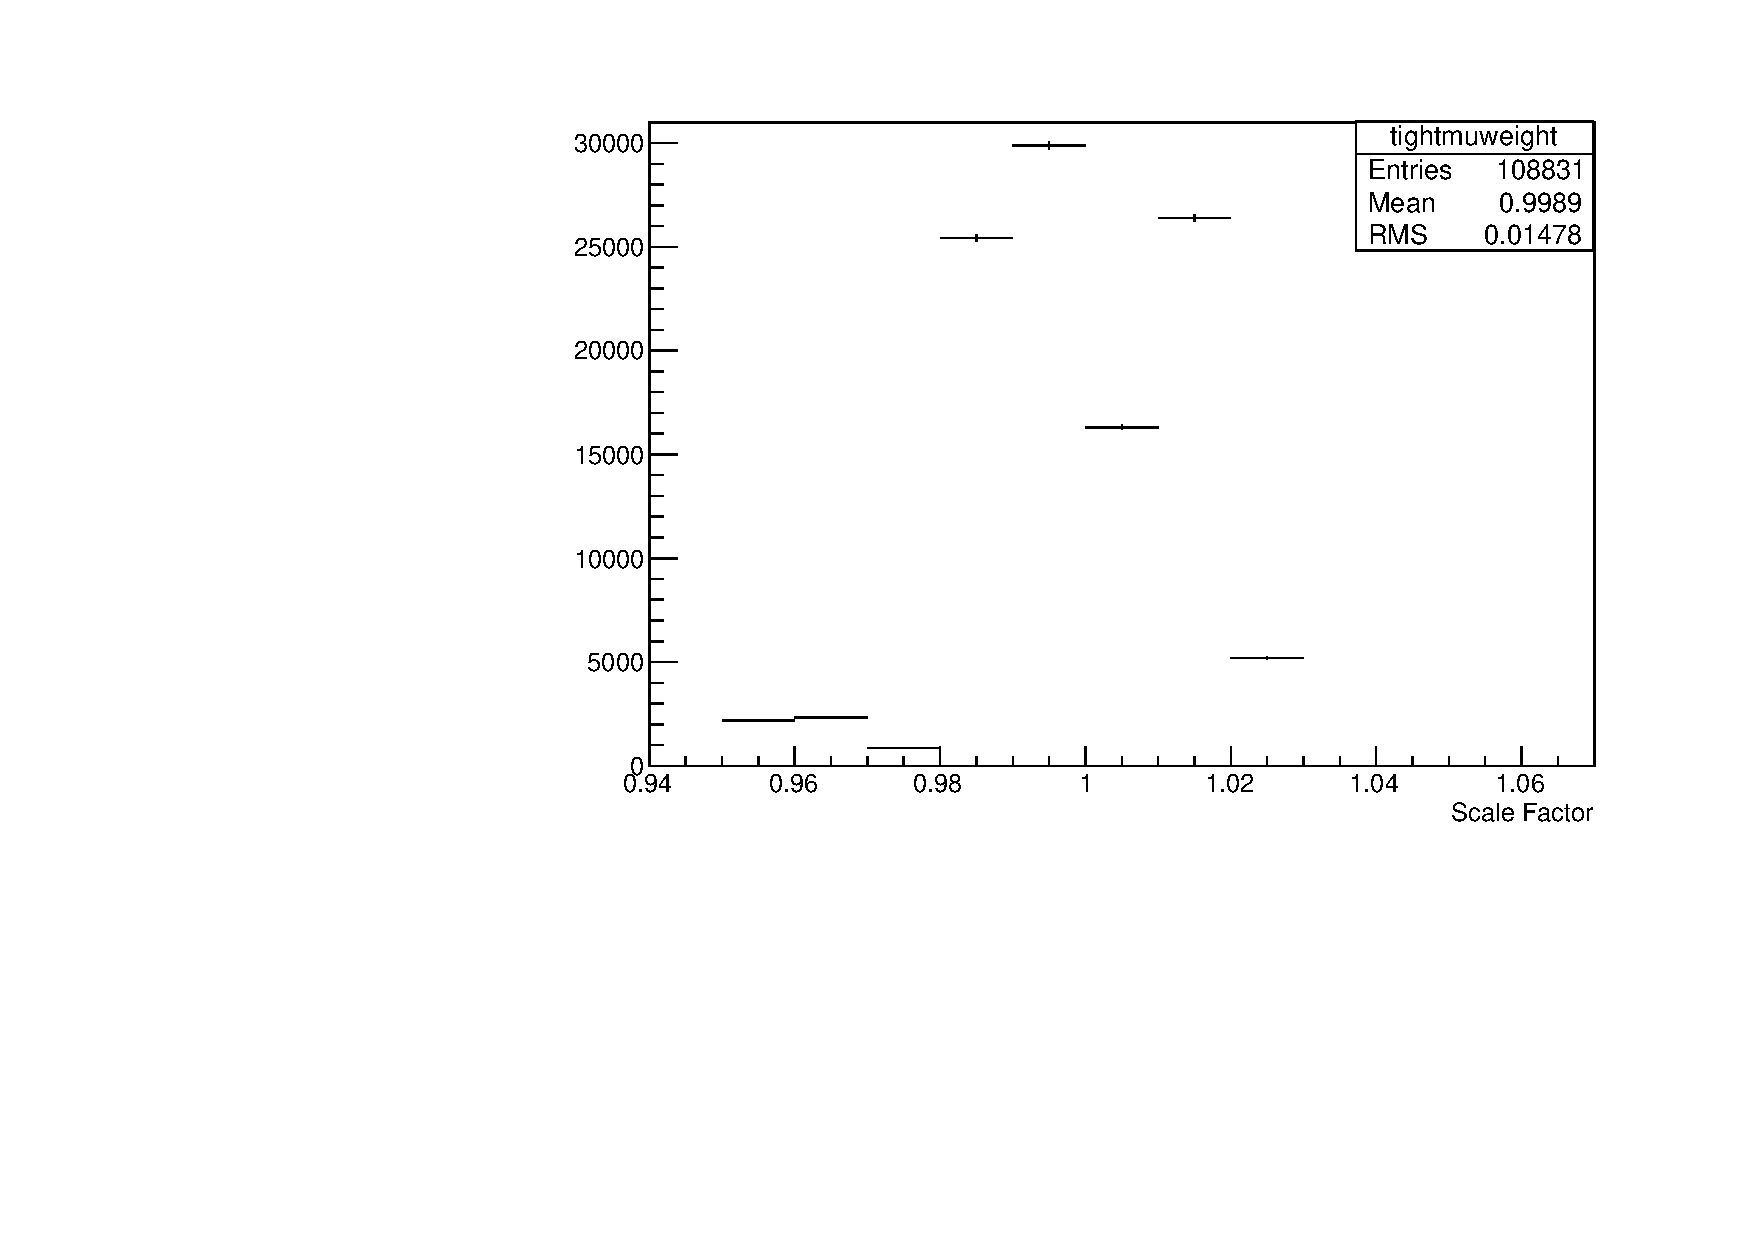
\includegraphics[width=1.1\textwidth]{TalkPics/lepeff141013/tight_muonweight_munu_munu.pdf}
  \end{columns}
  Plots after lepton selection step
\end{frame}

\begin{frame}\label{lastframe}
  \frametitle{Yields}
  \begin{block}{}
    \centering
    \footnotesize
    \begin{tabular}{|l|c|c|c|c|}
      \hline
      Channel & No correction & Central & Lep. eff. up & Lep. eff. down \\
      \hline
      $W\rightarrow e \nu$ & 68.8 (-4\%) & 71.8 & 71.5 (-0.4\%) & 72.1 (+0.4\%) \\
      $W\rightarrow\mu\nu$ & 67.4 (-1\%) & 68.1 & 66.3 (-2.6\%) & 69.1 (+1.5\%) \\
      \hline
    \end{tabular}
  \end{block}
\end{frame}


\end{fmffile}
\end{document}
